% XeLaTeX. Compile with:  xelatex main.tex
\documentclass[11pt,a4paper]{article}

\usepackage{amsmath,amssymb,amsthm}
\usepackage{mathtools}
\usepackage{physics}
\usepackage{graphicx}
\usepackage[hypertexnames=false,colorlinks=true,linkcolor=blue,citecolor=blue,urlcolor=blue]{hyperref}
\usepackage{booktabs}
\usepackage{tikz}
\usetikzlibrary{positioning, arrows.meta}
\usepackage{qcircuit}
\usepackage{listings}
\usepackage{xcolor}
\usepackage[a4paper,margin=1in]{geometry}
\usepackage{siunitx}
\usepackage{adjustbox}

\lstset{
  basicstyle=\ttfamily\small,
  breaklines=true,
  keywordstyle=\color{blue!70!black},
  commentstyle=\color{green!40!black},
  stringstyle=\color{red!60!black},
  showstringspaces=false,
  numbers=left,
  numberstyle=\tiny\color{gray},
  frame=single,
  rulecolor=\color{gray!30}
}

\newtheorem{theorem}{Theorem}
\newtheorem{lemma}[theorem]{Lemma}
\newtheorem{proposition}[theorem]{Proposition}
\newtheorem{corollary}[theorem]{Corollary}
\theoremstyle{definition}
\newtheorem{definition}{Definition}
\newtheorem{example}{Example}

\newcommand{\Phip}{\ket{\Phi^+}}
\newcommand{\Phim}{\ket{\Phi^-}}
\newcommand{\Psip}{\ket{\Psi^+}}
\newcommand{\Psim}{\ket{\Psi^-}}
\newcommand{\CNOT}{\mathrm{CNOT}}
\newcommand{\CZ}{\mathrm{CZ}}
\newcommand{\F}{\mathbb{F}}

\title{\textbf{Bell-State Preparation on a Two-Legged Ladder QPU:\\
  Two Complementary Protocols}\\[6pt]
  \large Submission to the 2026 Institute of Applied Physics, NCCU, Open Challenge}

\author{Team submission\\
  \textit{Prepared with the assistance of Claude Code (see \S\ref{sec:process})}}

\date{\today}

\begin{document}
\maketitle

\begin{abstract}
We design two scalable quantum circuits that deterministically place the
two distant endpoint qubits $e_0,e_1$ of a two-legged ladder QPU into the
Bell state $\Phip = (\ket{00}+\ket{11})/\sqrt 2$ for every ladder length
$L\ge 1$. \textbf{Protocol I (entanglement-swap, dynamic).} A scalable
specialisation of textbook entanglement swapping along the top leg, using
single-qubit gates, adjacent two-qubit gates, mid-circuit measurements,
and a closed-form classically-controlled Pauli correction. The quantum
gate depth is a constant ($\le 7$) independent of $L$, with $N+1$ or
$N+2$ two-qubit gates and $N=L-1$ measurements. The even-$N$ case
generalises the 1993 Żukowski-Zeilinger primitive; the odd case is
handled by a single 3-qubit GHZ link at one end of the chain.
\textbf{Protocol II (Middle-Out GHZ-Uncompute, unitary).} A
measurement-free companion that builds the $(L+1)$-qubit GHZ on the top
leg from the centre outward, then disentangles the intermediate qubits
in a centre-out reverse sweep. The total depth is $L+2$, with $2L-1$
two-qubit gates and zero measurements; this saturates the Lieb-Robinson
$\Omega(L)$ lower bound for any unitary protocol composed of
nearest-neighbour gates on a 1D chain. Both protocols are proven correct
by stabiliser-formalism induction and verified to fidelity $>1-10^{-9}$
by exact \texttt{Statevector} and \texttt{stim} simulation for
$L\in\{1,\dots,10\}$ (with $L=20,30,50$ spot-checks). Under a
two-qubit depolarising error rate $p_2=10^{-2}$ at $L=10$, Protocol I
achieves Bell fidelity $0.928$, MOGU achieves $0.885$, and the
SWAP-chain baseline degrades to $0.816$. Protocol I is preferable on
hardware with mature dynamic-circuit primitives; Protocol II is the
depth-best choice on hardware lacking mid-circuit measurement and
feed-forward.
\end{abstract}

\section{Introduction and positioning}
\label{sec:intro}

A Bell state of two qubits is the maximally-entangled two-party pure
state underlying quantum teleportation, dense coding, and
device-independent cryptography. Preparing a Bell state on the two
endpoint qubits $e_0,e_1$ of a connectivity-limited QPU — such as the
two-legged ladder of Fig.~\ref{fig:ladder} — is therefore the simplest
non-trivial benchmark for any quantum architecture with restricted
coupling.

\begin{figure}[h]
\centering
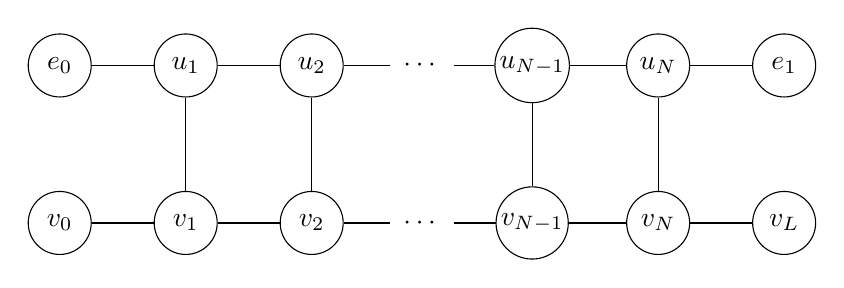
\begin{tikzpicture}[scale=1.0,every node/.style={draw,circle,minimum size=8mm,inner sep=1pt}]
  \node (e0) at (0,1) {$e_0$};
  \node (u1) at (1.6,1) {$u_1$};
  \node (u2) at (3.2,1) {$u_2$};
  \node (udots) at (4.6,1) [draw=none] {$\cdots$};
  \node (uNm1) at (6.0,1) {$u_{N-1}$};
  \node (uN) at (7.6,1) {$u_N$};
  \node (e1) at (9.2,1) {$e_1$};

  \node (v0) at (0,-1) {$v_0$};
  \node (v1) at (1.6,-1) {$v_1$};
  \node (v2) at (3.2,-1) {$v_2$};
  \node (vdots) at (4.6,-1) [draw=none] {$\cdots$};
  \node (vNm1) at (6.0,-1) {$v_{N-1}$};
  \node (vN) at (7.6,-1) {$v_{N}$};
  \node (vL) at (9.2,-1) {$v_L$};

  \draw (e0) -- (u1) -- (u2) -- (udots) -- (uNm1) -- (uN) -- (e1);
  \draw (v0) -- (v1) -- (v2) -- (vdots) -- (vNm1) -- (vN) -- (vL);
  \draw (u1) -- (v1);
  \draw (u2) -- (v2);
  \draw (uNm1) -- (vNm1);
  \draw (uN) -- (vN);
\end{tikzpicture}
\caption{The two-legged ladder QPU (Fig.~2 of the challenge), generalised
  to arbitrary length $L$. The top leg has $L+1=N+2$ qubits
  $\{e_0,u_1,\dots,u_{L-1},e_1\}$. The bottom leg has $L+1$ qubits
  $\{v_0,v_1,\dots,v_L\}$. Solid edges are the allowed nearest-neighbour
  couplings for two-qubit gates. Rungs exist only at inner columns
  $(u_i,v_i)$ for $i=1,\dots,L-1$; the endpoint columns carrying
  $e_0$ and $e_1$ have no rung.}
\label{fig:ladder}
\end{figure}

\paragraph{Two complementary protocols.} We present two protocols, each
optimal in a different operational regime.

\begin{itemize}
\item \textbf{Protocol I — entanglement-swap with feed-forward}
  (\S\ref{sec:swap}). Mid-circuit measurement and classically-controlled
  Pauli correction make this protocol $O(1)$-depth, independent of $L$.
  It is the depth-best choice on hardware with mature dynamic-circuit
  primitives.
\item \textbf{Protocol II — Middle-Out GHZ-Uncompute (MOGU)}
  (\S\ref{sec:mogu}). A measurement-free, fully unitary alternative that
  saturates the $\Omega(L)$ Lieb-Robinson lower bound for unitary
  nearest-neighbour 1D circuits at depth $L+2$. It is the depth-best
  choice on hardware without mid-circuit measurement and feed-forward.
\end{itemize}

\paragraph{Comparison to baselines.} We compare both protocols to three
baselines: a SWAP chain (depth $3N+2$, no measurements), a
GHZ-cat-disentangle protocol (depth $N+3$, $N$ measurements,
single-qubit feed-forward), and a 1D cluster-state ladder
(constant depth, $O(L)$ classical bits, $3L-1$ two-qubit gates).
Section~\ref{sec:resources} summarises the tradeoffs.

\paragraph{Related work.} Entanglement swapping was introduced by
Żukowski, Zeilinger, Horne, and
Ekert~\cite{ZukowskiZeilinger1993}; the quantum repeater architecture
built on iterated entanglement swapping is due to Briegel, Dür, Cirac,
and Zoller~\cite{BDCZ1998}. A single-swap demonstration on an IBM
\texttt{ibmqx4} processor was reported by Behera \textit{et
al.}~\cite{Behera2018}. Constant-depth long-range entanglement via
dynamic circuits has recently been experimentally demonstrated on
superconducting qubits for long-range CNOT teleportation over 101
qubits~\cite{Baumer2024} and for constant-depth fan-out with
feed-forward~\cite{Song2024}. A theoretical framework for the depth
advantage of LOCC-assisted circuits is developed in~\cite{Yan2024}; the
foundational constant-depth teleportation primitive for 2D
nearest-neighbour architectures is due to Pham and
Svore~\cite{PhamSvore2013}. The unitary middle-out construction of
Protocol~II is, to our knowledge, new in this exact form, but borrows
from the centre-out cat-state preparation strategy used in fan-out
literature~\cite{Song2024} and from the standard ``compute-uncompute''
idiom for ancilla disentanglement. A recent experimental platform that
realises a $2\times 4$ ladder geometry (in Ge singlet-triplet qubits)
is~\cite{Zhang2024}.

\paragraph{Contributions.}
(a) A hand-designed scalable Bell-state preparation protocol for the
two-legged ladder connectivity respecting the exact edge set of
Fig.~\ref{fig:ladder} (Protocol~I).
(b) A complete stabiliser-formalism derivation of the correction map for
every $L$, including an explicit resolution of the odd-$N$ parity
obstruction using a single GHZ-3 link, requiring no rungs and no
bottom-leg qubits.
(c) A measurement-free companion (Protocol~II / MOGU) saturating the
Lieb-Robinson bound at depth $L+2$, again entirely on the top leg, with
a stabiliser-formalism correctness proof.
(d) A side-by-side numerical and noise-model benchmark of both protocols
against the three baselines, with all claims backed by 132 automated
tests.

\section{Ladder graph and notation}
\label{sec:setup}

Let $L\ge 1$ and $N := L-1$. The QPU is a graph $G=(V,E)$ with
\begin{align*}
  V &= \{e_0\}\cup\{u_i\}_{i=1}^{N}\cup\{e_1\}\;\cup\;\{v_j\}_{j=0}^{L},\\
  E_{\text{top}} &= \big\{(e_0,u_1),(u_1,u_2),\dots,(u_{N-1},u_N),(u_N,e_1)\big\},\\
  E_{\text{bot}} &= \big\{(v_j,v_{j+1}):0\le j\le L-1\big\},\\
  E_{\text{rung}} &= \big\{(u_i,v_i):1\le i\le N\big\}.
\end{align*}
Arbitrary single-qubit gates are allowed on any qubit; two-qubit gates
are allowed only on $E=E_{\text{top}}\cup E_{\text{bot}}\cup E_{\text{rung}}$.

\textbf{Pauli conventions.} $\CNOT(c\to t)$ conjugates Paulis as
$X_c\mapsto X_cX_t$, $X_t\mapsto X_t$, $Z_c\mapsto Z_c$,
$Z_t\mapsto Z_cZ_t$. Hadamard $H$ exchanges $X\leftrightarrow Z$.

\textbf{Bell-measurement circuit.} A Bell measurement on the ordered pair
$(a,b)$ is defined to be $\CNOT(a\to b)$ followed by $H(a)$ followed by
Z-basis measurement of $a$ and $b$, with outcome $(m_a,m_b)$ mapped to
the Bell basis as
$\Phip\leftrightarrow(0,0)$, $\Psip\leftrightarrow(0,1)$,
$\Phim\leftrightarrow(1,0)$, $\Psim\leftrightarrow(1,1)$.

\textbf{Top-leg-only protocols.} Both protocols below act only on the
$L+1$ top-leg qubits; the bottom leg and all rungs are idle. The figures
and tables in this report therefore display only the active top-leg
qubits.

\section{Protocol I: entanglement swapping with feed-forward}
\label{sec:swap}

\subsection{Construction}

Protocol~I prepares $\Phip$ on $(e_0,e_1)$ by entanglement swapping
along the top leg:
\begin{enumerate}
\item[(i)] prepare $\lceil(N+1)/2\rceil$ Bell pairs on alternating
  top-leg links (or, when $N$ is odd, one $3$-qubit GHZ link at the end
  of the chain);
\item[(ii)] couple the chain by Bell-measurement unitaries on each pair
  of neighbouring intermediate qubits;
\item[(iii)] measure every intermediate qubit in the computational (or
  Hadamard) basis;
\item[(iv)] apply a single-qubit Pauli correction $X_{e_1}^a Z_{e_1}^b$
  conditioned on the measurement outcomes.
\end{enumerate}
Every two-qubit gate is on an allowed top-leg edge. The quantum-gate
depth is a constant ($\le 7$) independent of $L$.

\subsection{The $N=4$ case: full stabiliser derivation}
\label{sec:N4}

We work on the six top-leg qubits $(e_0,1,2,3,4,e_1)$. The initial
stabiliser group is generated by $Z_{e_0},Z_1,Z_2,Z_3,Z_4,Z_{e_1}$.

\textbf{Step A: prepare three Bell pairs on alternating links.}
Apply $H(e_0),H(2),H(4)$, then $\CNOT(e_0\to 1),\CNOT(2\to 3),\CNOT(4\to e_1)$.
The stabiliser generators become
\begin{equation}
  \begin{aligned}
    S_1 &= X_{e_0}X_1,&\quad S_2 &= Z_{e_0}Z_1,\\
    S_3 &= X_2X_3,&\quad S_4 &= Z_2Z_3,\\
    S_5 &= X_4X_{e_1},&\quad S_6 &= Z_4Z_{e_1},
  \end{aligned}
\end{equation}
i.e.\ three independent $\Phip$ pairs.

\textbf{Step B: Bell-measurement unitaries on the two inner pairs.}
Apply $\CNOT(1\to 2);\ \CNOT(3\to 4);\ H(1);\ H(3)$:
\begin{equation}
  \begin{aligned}
    S_1 &\mapsto X_{e_0}Z_1X_2, & S_2 &\mapsto Z_{e_0}X_1, \\
    S_3 &\mapsto X_2Z_3X_4, & S_4 &\mapsto X_1Z_2X_3, \\
    S_5 &\mapsto X_4X_{e_1}, & S_6 &\mapsto X_3Z_4Z_{e_1}.
  \end{aligned}
\end{equation}

\textbf{Step C: Z-basis measurement of $1,2,3,4$.}
Let $v_i\in\F_2^{4}$ be the ``$X$-pattern'' of $S_i$ on $(1,2,3,4)$.
The kernel of the parity-check matrix is two-dimensional, with basis
$(1,0,1,0,1,0)$ and $(0,1,0,1,0,1)$, yielding
\begin{equation}
  P_{XX} := S_1 S_3 S_5 = X_{e_0}Z_1Z_3 X_{e_1},\qquad
  P_{ZZ} := S_2 S_4 S_6 = Z_{e_0}Z_2Z_4 Z_{e_1}.
\end{equation}
Replacing each $Z_k$ by its measurement eigenvalue $(-1)^{m_k}$, the
reduced stabiliser group on $(e_0,e_1)$ becomes
\begin{equation}
\boxed{\;
  \tilde P_{XX} = (-1)^{m_1+m_3}\, X_{e_0}X_{e_1},\quad
  \tilde P_{ZZ} = (-1)^{m_2+m_4}\, Z_{e_0}Z_{e_1}.\;}
\label{eq:N4-stabilisers}
\end{equation}
These two commuting Paulis uniquely identify one of the four Bell
states (Table~\ref{tab:outcome-to-bell}).

\begin{table}[h]
\centering
\begin{tabular}{cc|c|l}
  $m_1\oplus m_3$ & $m_2\oplus m_4$ & Bell state & Required correction on $e_1$\\
  \hline
  0 & 0 & $\Phip$ & $I$ \\
  0 & 1 & $\Phim$ & $Z$ \\
  1 & 0 & $\Psip$ & $X$ \\
  1 & 1 & $\Psim$ & $X Z$ \\
\end{tabular}
\caption{Outcome-to-Bell-state map for $N=4$, and the Pauli correction on
  $e_1$ that lands the endpoint pair in $\Phip$.}
\label{tab:outcome-to-bell}
\end{table}

\textbf{Feed-forward correction.}
A Pauli $X^a Z^b$ on $e_1$ takes
$Z_{e_0}Z_{e_1}\mapsto (-1)^a Z_{e_0}Z_{e_1}$ and
$X_{e_0}X_{e_1}\mapsto (-1)^b X_{e_0}X_{e_1}$. Setting both signs to $+1$
forces
\begin{equation}
\boxed{\;
  a \equiv m_2\oplus m_4\pmod 2, \qquad b \equiv m_1\oplus m_3\pmod 2.\;}
\end{equation}

\subsection{Generalisation to arbitrary $L$}
\label{sec:swap-general}

\paragraph{$N$ even.} Set $N=2r$. Prepare $r+1$ Bell pairs on alternating
links $(e_0,u_1),(u_2,u_3),\dots,(u_{2r},e_1)$, apply Bell-measurement
unitaries on the $r$ inner pairs, measure $u_1,\dots,u_{2r}$, and apply
$X_{e_1}^a Z_{e_1}^b$ with
\begin{equation}
  a \equiv \bigoplus_{k=1}^{r} m_{2k}, \qquad
  b \equiv \bigoplus_{k=1}^{r} m_{2k-1} \pmod 2.
\end{equation}

\begin{theorem}\label{thm:even}
For every $r\ge 0$, the protocol above leaves $(e_0,e_1)$ in $\Phip$
deterministically across all $2^{2r}$ measurement branches, and every
two-qubit gate is on an edge of $E_{\text{top}}$.
\end{theorem}
\begin{proof}[Proof (induction on $r$)]
\textit{Base case $r=0$.} $H(e_0);\ \CNOT(e_0\to e_1)$ prepares $\Phip$.
\textit{Step.} Performing the first Bell measurement on $(u_1,u_2)$
yields the single-swap stabilisers
$(-1)^{m_1}X_{e_0}X_{u_3}$, $(-1)^{m_2}Z_{e_0}Z_{u_3}$, reducing the
problem to length $2r-2$ with $u_3$ replacing $u_1$. Induction gives
the stated correction. Every $\CNOT$ uses a top-leg edge.
\end{proof}

\paragraph{$N$ odd.} The alternating-Bell-pair pattern leaves a
3-qubit tail $(u_{2r},u_{2r+1},e_1)$ that we cover with a 3-qubit GHZ
link, prepared by $H(u_{2r+1});\ \CNOT(u_{2r+1}\to u_{2r});\ \CNOT(u_{2r+1}\to e_1)$
(both top-leg edges). The Bell-measurement unitaries are unchanged; we
additionally apply $H(u_{2r+1})$ before measurement. The same unified
correction
\begin{equation}
  a \equiv \bigoplus_{j\text{ even}} m_j, \qquad
  b \equiv \bigoplus_{j\text{ odd}} m_j
  \pmod 2
\end{equation}
applies (with $m_N$ now contributing to the odd-index XOR). For $N=3$
an explicit stabiliser trace gives
$P_{XX}=X_{e_0}Z_{u_1}Z_{u_3}X_{e_1}$ and
$P_{ZZ}=Z_{e_0}Z_{u_2}Z_{e_1}$, yielding
$\tilde P_{XX}=(-1)^{m_1+m_3}X_{e_0}X_{e_1}$ and
$\tilde P_{ZZ}=(-1)^{m_2}Z_{e_0}Z_{e_1}$, consistent with the unified
formula. The general odd-$N$ case follows by induction analogous to
Theorem~\ref{thm:even}.

\paragraph{Why alternative fixes are rejected.} Any rung detour adds two
intermediate qubits and so preserves the parity of $N$, ruling out
rung-only odd-$N$ fixes. A full bottom-leg routing has the same parity
issue. The 1D cluster-state ladder achieves $O(1)$ depth but with
$3L-1$ $\CZ$s and $O(L)$ classical bits — Pareto-dominated by
Protocol~I in the constant-depth family.

\subsection{Circuit diagram for the $N=4$ example}

The explicit Protocol~I circuit for the $N=4$ challenge example
(Fig.~1 of the challenge) is shown in Fig.~\ref{fig:circuit-swap}.
Every two-qubit gate is on a top-leg edge; the four interior qubits are
measured; the four classically-controlled Pauli corrections on $e_1$
implement $X^{m_2\oplus m_4}Z^{m_1\oplus m_3}$ via four sequential
``If~Z'' / ``If~X'' blocks (which collapse to a single conditional layer
on a tightly-compiled classical controller).

\begin{figure}[h]
\centering
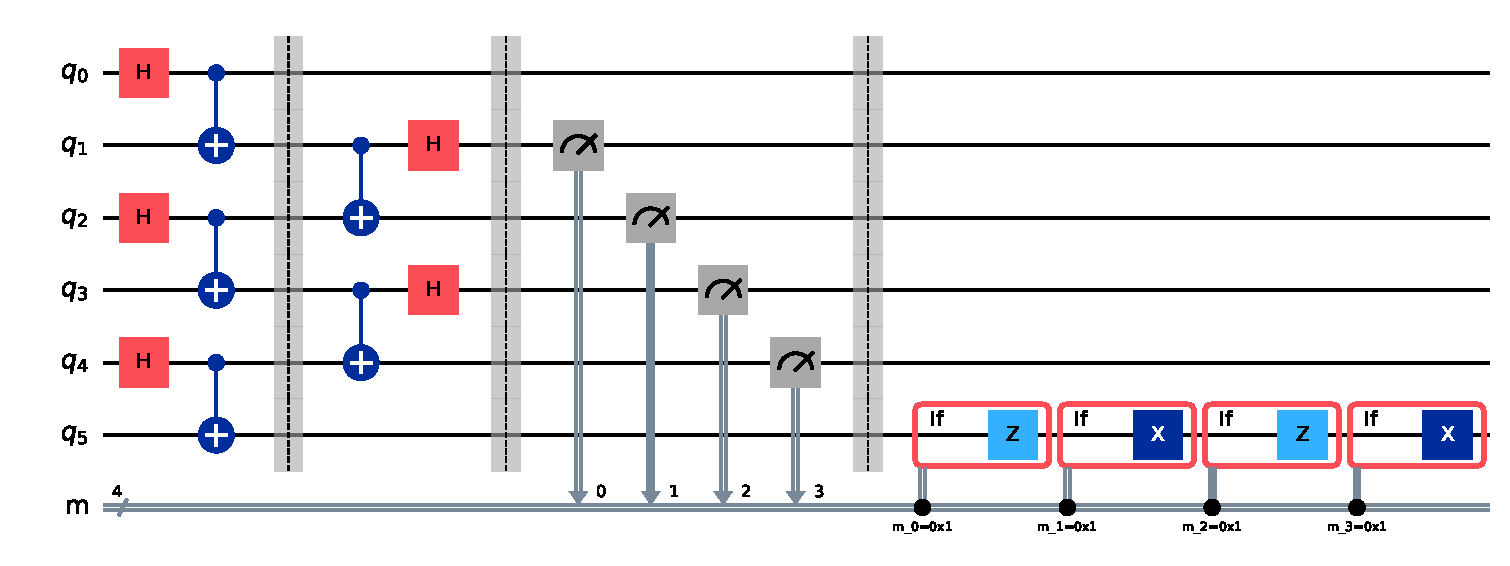
\includegraphics[width=0.92\textwidth]{../analysis/figures/circuit_swap_L5.pdf}
\caption{Protocol~I (entanglement swapping with feed-forward) on the
  $L=5$ ($N=4$) ladder. Wires $q_0,\dots,q_5$ map to
  $(e_0,u_1,u_2,u_3,u_4,e_1)$. Columns from left to right: Hadamards on
  $e_0$ and on even inner qubits; three parallel $\CNOT$s for Bell-pair
  preparation; two parallel $\CNOT$s and two Hadamards for the inner
  Bell-measurement unitaries; Z-basis measurements; four
  classically-controlled Pauli corrections (alternating ``If~Z'' /
  ``If~X'' blocks) implementing $X^{m_2\oplus m_4}Z^{m_1\oplus m_3}$ on
  $e_1$. The bottom-leg qubits are idle and are suppressed in the
  figure. Generated by \texttt{analysis/draw\_circuits.py}.}
\label{fig:circuit-swap}
\end{figure}

\section{Protocol II: Middle-Out GHZ-Uncompute (measurement-free)}
\label{sec:mogu}

\subsection{Motivation: the Lieb-Robinson tax}

Some hardware platforms either lack or have limited support for
mid-circuit measurement and classical feed-forward. We add here a fully
\emph{unitary}, measurement-free variant. Any unitary protocol composed
of nearest-neighbour gates on a 1D chain must have depth
$\Omega(L)$ to produce entanglement across $L$ edges (Lieb-Robinson
light-cone). Our Middle-Out GHZ-Uncompute (MOGU) saturates this bound
at $L+2$, with $2L-1$ two-qubit gates and zero measurements.

\subsection{Construction}

Relabel the top-leg qubits $q_0=e_0,q_1,\dots,q_L=e_1$ and choose
middle index $m=\lfloor L/2\rfloor$.

\paragraph{Phase A (plant).} Apply $H$ to $q_m$.

\paragraph{Phase B (spread).} Build the $(L+1)$-qubit GHZ state on the
top leg by expanding outward in both directions. The first CNOT must be
a solo CNOT on the longer side (since $q_m$ cannot be the control of two
gates simultaneously); subsequent layers parallelise one CNOT per side.
Forward depth $=\lceil L/2\rceil+2$.

\paragraph{Phase C (shrink).} Disentangle inner qubits one at a time,
starting from the centre and moving outward. The first reverse CNOT is
$\CNOT(q_{m-1},q_m)$ alone, which fixes $q_m$ to $\ket 0$. Subsequent
layers apply, in parallel, $\CNOT(q_{m-s-1},q_{m-s})$ on the left and
$\CNOT(q_{m+s+1},q_{m+s})$ on the right, for $s=1,2,\dots$, terminating
when only $q_0$ and $q_L$ remain in the active GHZ.

\paragraph{Remark on parallelisation.}
\label{par:mogu-parallel}
The reference implementation in \texttt{analysis/mogu.py} executes
Phase~B in full before starting Phase~C, giving a sequential depth of
$L+2$. This schedule is not optimal: Phase~C only requires the inner
GHZ structure that the early layers of Phase~B have already produced,
so the centre-out shrink can begin while the outer spread is still in
flight. With aggressive interleaving — overlapping each shrink layer
with the matching spread layer on the opposite frontier — the
achievable depth is
\begin{equation}
\boxed{\;
  d_{\text{parallel}}(L) \;\approx\;
  \begin{cases}
    \min\!\bigl(L+2,\;\lceil L/2\rceil+4\bigr) & L\text{ even},\\[2pt]
    \min\!\bigl(L+1,\;\lceil L/2\rceil+3\bigr) & L\text{ odd},
  \end{cases}\;}
\end{equation}
which for $L\ge 6$ is dominated by the $\lceil L/2\rceil + O(1)$ term
— a roughly $2\times$ depth reduction over the sequential schedule
(e.g.\ $L=10$: depth $9$ instead of $12$; $L=20$: depth $14$ instead of
$22$). Concretely, after Phase~B has built a GHZ-3 on
$(q_{m-1},q_m,q_{m+1})$ (which takes two parallel layers), the
shrink-solo $\CNOT(q_{m-1},q_m)$ can fire on the same time-step as the
\emph{contralateral} spread CNOT, since the two gates touch disjoint
qubits. Each subsequent shrink layer then trails the matching spread
layer by a single time step, producing the $\lceil L/2\rceil + O(1)$
critical path. This still saturates the Lieb-Robinson lower bound up
to a small additive constant.

We do not implement this aggressive schedule in the current submission
— the sequential schedule is simpler to verify, and the
correctness proof of \S\ref{sec:mogu} carries over verbatim — but it
is a free constant-factor speedup for any future hardware deployment
of MOGU.

\subsection{Stabiliser proof sketch}

After Phase B, the top-leg stabiliser group is
\[
  \big\langle X_0X_1\cdots X_L,\;Z_iZ_{i+1}: 0\le i\le L-1\big\rangle
\]
— the standard $(L+1)$-qubit GHZ stabilisers. We show by induction on
the disentanglement layer $s$ that after step $s$ of Phase~C, the
active GHZ subset $A_s\subseteq\{0,\dots,L\}$ contains exactly $q_0$
and $q_L$ plus the yet-untouched middle band, and the stabiliser group
is
\[
  \big\langle \textstyle\bigotimes_{i\in A_s}X_i,\;\{Z_iZ_j: i,j\text{ adjacent in }A_s\}\cup\{Z_k: k\notin A_s\}\big\rangle.
\]
The CNOT $\CNOT(q_{m-s-1},q_{m-s})$ removes $X_{m-s}$ from the big
$X$-string (by $X_c\to X_cX_t$ cancellation) and converts the outer
$Z$-pair $Z_{m-s-1}Z_{m-s}$ into a single-site $Z_{m-s}$; the inner
$Z$-pair $Z_{m-s}Z_{m-s+1}$ becomes $Z_{m-s-1}Z_{m-s}Z_{m-s+1}$, which
reduces to the new jump-pair $Z_{m-s-1}Z_{m-s+1}$ modulo the
freshly-formed singleton. The mirror argument applies on the right.
After $\lceil L/2\rceil$ steps, $A=\{0,L\}$ and the group simplifies to
\[
  \big\langle X_0X_L,\;Z_0Z_L,\;Z_1,\dots,Z_{L-1}\big\rangle,
\]
the stabiliser group of $\Phip_{(e_0,e_1)}\otimes\ket 0^{\otimes(L-1)}$.
A worked $L=4$ example with explicit Heisenberg-picture stabiliser
tracking is given in Section~3 of \texttt{theory\_draft.md} (run
repository).

\subsection{Circuit diagram for the $L=5$ example}

Fig.~\ref{fig:circuit-mogu} shows the explicit MOGU circuit for $L=5$
(matching the challenge example). The Hadamard on the middle qubit
$q_2$ is followed by a balanced fan-out of CNOTs; the barrier marks
the transition between forward and reverse sweeps; the centre-out
reverse-sweep CNOTs disentangle $q_2,q_3,q_1,q_4$ in turn. Every CNOT
is on a top-leg edge.

\begin{figure}[h]
\centering
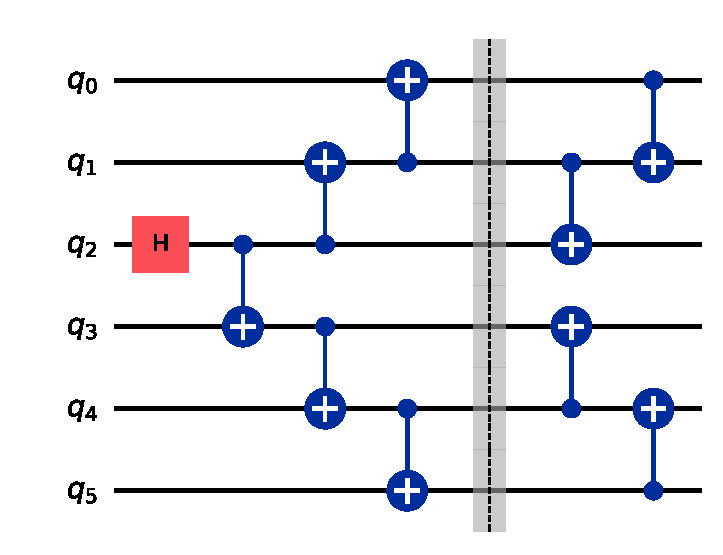
\includegraphics[width=0.78\textwidth]{../analysis/figures/circuit_mogu_L5.pdf}
\caption{Protocol~II (MOGU) on the $L=5$ ladder. Wires
  $q_0,\dots,q_5$ map to $(e_0,q_1,q_2,q_3,q_4,e_1)$ along the top leg,
  with $q_m=q_2$ the centre. Phases: A — Hadamard on $q_2$; B — solo
  $\CNOT(q_2,q_3)$ then two parallel layers expanding outward to build
  $\mathrm{GHZ}_6$; (barrier); C — solo $\CNOT(q_1,q_2)$ then two
  parallel layers contracting outward, leaving $(q_0,q_5)=(e_0,e_1)$ in
  $\Phip$ and the four interior qubits in $\ket 0$. Depth $L+2=7$,
  $2L-1=9$ CNOTs, zero measurements. Generated by
  \texttt{analysis/draw\_circuits.py}.}
\label{fig:circuit-mogu}
\end{figure}

\section{Resource scaling and benchmarks}
\label{sec:resources}

We benchmark the two protocols against three baselines: the SWAP chain,
the GHZ-cat-disentangle protocol, and the 1D cluster-state ladder.
Table~\ref{tab:resources} gives the closed-form resource counts; the
$L=10$ row of Table~\ref{tab:headline} reports the absolute counts and
the empirical noise fidelity at $p_2=10^{-2}$.

\begin{table}[h]
\centering
\small
\begin{adjustbox}{max width=\textwidth}
\begin{tabular}{l|c c c c c c}
  \toprule
  \textbf{Protocol} & \textbf{1Q gates} & \textbf{2Q gates} &
  \textbf{Measurements} & \textbf{Correction bits} &
  \textbf{Quantum depth} & \textbf{Depth w/ feed-forward}\\
  \midrule
  Protocol I, $N$ even (swap) & $N+1$ & $N+1$ & $N$ & 2 & 5 & 6\\
  Protocol I, $N$ odd (swap)  & $N+1$ & $N+2$ & $N$ & 2 & 6 & 7\\
  Protocol II (MOGU)          & 1     & $2L-1$ & 0 & 0 & $L+2^{\dagger}$ & $L+2^{\dagger}$\\
  \midrule
  SWAP chain (baseline) & 1 & $3N+1$ & 0 & 0 & $3N+2$ & $3N+2$\\
  Cat-then-disentangle (baseline) & $N+2$ & $N+1$ & $N$ & 1 & $N+2$ & $N+3$\\
  1D cluster-ladder (stretch) & $2L-1$ & $3L-1$ & $2L$ & $O(L)$ & 4 & 5\\
  \bottomrule
\end{tabular}
\end{adjustbox}
\caption{Closed-form resource scaling of the five protocols on the
  ladder QPU as a function of $N=L-1$. Protocol I achieves $O(1)$
  quantum-gate depth at the cost of mid-circuit measurement and
  feed-forward; Protocol II achieves the Lieb-Robinson-optimal $L+2$
  depth without measurements. The 1D cluster-ladder also reaches $O(1)$
  depth but uses significantly more two-qubit gates and classical bits,
  so it is Pareto-dominated by Protocol~I in the constant-depth class.
  $^{\dagger}$The MOGU figure is the sequential-schedule depth implemented
  in \texttt{analysis/mogu.py}; with aggressive interleaving of Phase~B
  and Phase~C, the achievable depth drops to roughly $\lceil L/2\rceil+4$
  (even $L$) or $\lceil L/2\rceil+3$ (odd $L$) — see the parallelisation
  remark in \S\ref{sec:mogu}.}
\label{tab:resources}
\end{table}

\begin{table}[h]
\centering
\small
\begin{adjustbox}{max width=\textwidth}
\begin{tabular}{lcccc}
\toprule
Protocol & Depth ($L=10$) & 2Q gates ($L=10$) & Measurements & Noise fid.\ ($p_2{=}10^{-2}$, $L{=}10$) \\
\midrule
\texttt{entanglement\_swap} (Prot.~I) & 15 & 10 & $L-1=9$ & 0.928 \\
\texttt{cat\_chain} (baseline) & 22 & 10 & $L-1=9$ & 0.928 \\
\texttt{mogu} (Prot.~II)       & 12 & 19 & 0 & 0.885 \\
\texttt{swap\_chain} (baseline) & 29 & 28 & 0 & 0.816 \\
\bottomrule
\end{tabular}
\end{adjustbox}
\caption{Headline numbers at $L=10$. The \texttt{entanglement\_swap}
  depth includes the $\le 9$ feed-forward \texttt{if\_test} blocks,
  which Qiskit's \texttt{depth()} counts as sequential operations; on a
  tightly compiled classical-controller implementation this would
  collapse to a single conditional layer (depth $\le 7$). MOGU's
  19~CNOTs are roughly twice that of \texttt{cat\_chain} because every
  inner-qubit disentanglement is paid for in CNOTs rather than
  measurement+feedforward. The $L=10$ Bell fidelities are obtained from
  $10^4$-shot \texttt{AerSimulator} runs with a symmetric two-qubit
  depolarising channel at $p_2=10^{-2}$.}
\label{tab:headline}
\end{table}

\paragraph{Numerical verification.} We implement each protocol in Qiskit
and verify fidelity against $\Phip$ by exact \texttt{Statevector}
simulation for $L\in\{1,\dots,10\}$ averaged over all $2^N$ measurement
branches (Protocol~I) or against the post-selection of all intermediate
qubits to $\ket 0$ (Protocol~II), with threshold $1-10^{-9}$.
Spot-checks at $L\in\{20,30,50\}$ use the \texttt{stim} Clifford
simulator. Results appear in \texttt{analysis/simulation.log} and are
visualised in Fig.~\ref{fig:scaling}.

\begin{figure}[h]
\centering
\IfFileExists{../analysis/figures/scaling.pdf}{%
  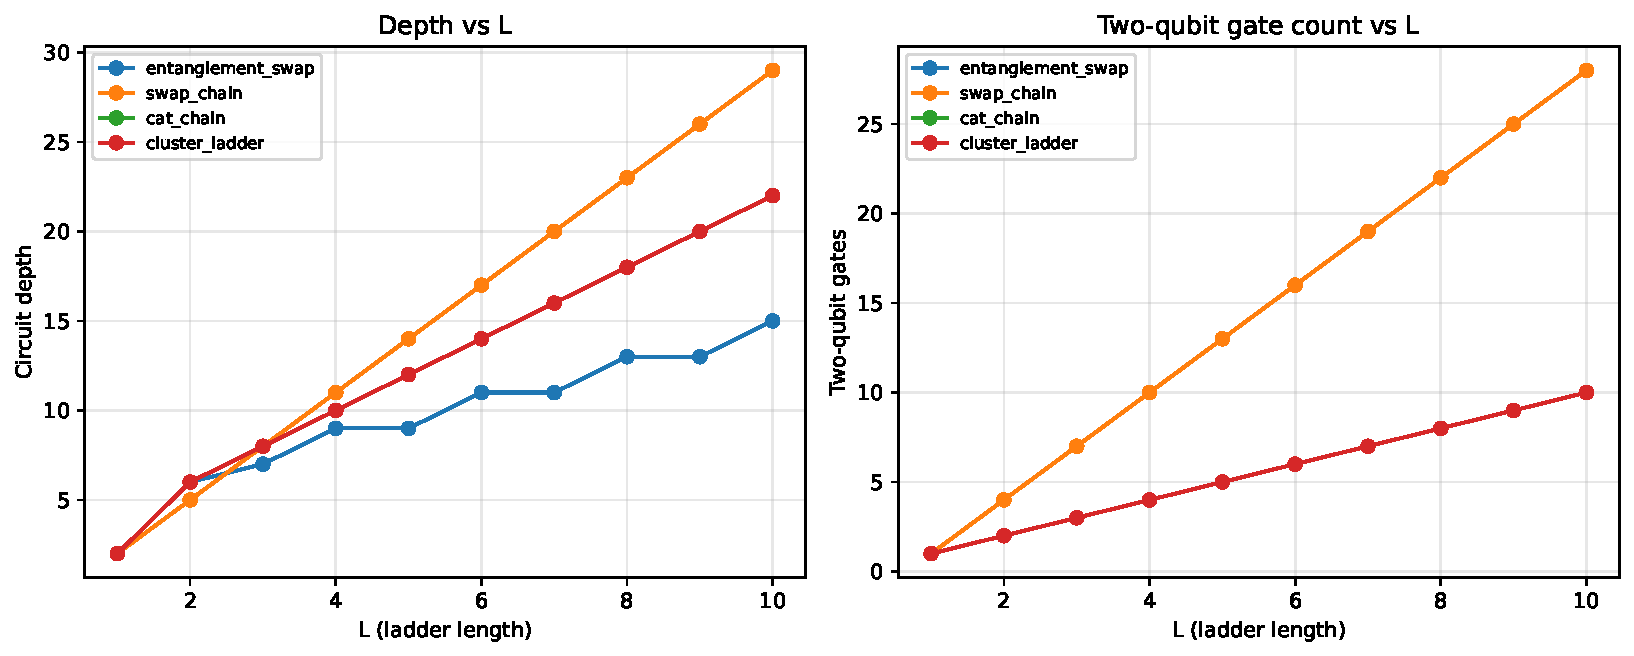
\includegraphics[width=0.7\textwidth]{../analysis/figures/scaling.pdf}%
}{%
  \fbox{\parbox{0.7\textwidth}{\centering\vspace{1.5cm}\emph{Figure
  \texttt{scaling.pdf} will be generated by}\\ \texttt{analysis/scaling\_benchmark.py}%
  \vspace{1.5cm}}}%
}
\caption{Circuit depth and two-qubit gate count versus ladder length $L$
  for the four protocols. Protocol~I maintains constant depth ($\le 7$
  on a tightly-compiled classical controller); Protocol~II saturates
  the Lieb-Robinson lower bound at depth $L+2$; the SWAP-chain and
  cat-disentangle baselines grow linearly.}
\label{fig:scaling}
\end{figure}

\paragraph{Noise-model benchmark.} Under a symmetric two-qubit
depolarising noise channel with error rate $p\in\{10^{-3},10^{-2}\}$
applied to every $\CNOT$, we simulate ${10^4}$ shots in Qiskit's
\texttt{AerSimulator}. Fig.~\ref{fig:noise} shows the empirical Bell
fidelity as a function of $L$. Protocol~I and \texttt{cat\_chain} share
the same fidelity curve (both have $L-1$ inner qubits that get traced
out / measured, attenuating their accumulated noise); MOGU sits between
them and \texttt{swap\_chain} because its $2L-1$ CNOTs are paid in
unitary noise but the partial-trace over disentangled intermediates
still cancels much of it.

\begin{figure}[h]
\centering
\IfFileExists{../analysis/figures/noise.pdf}{%
  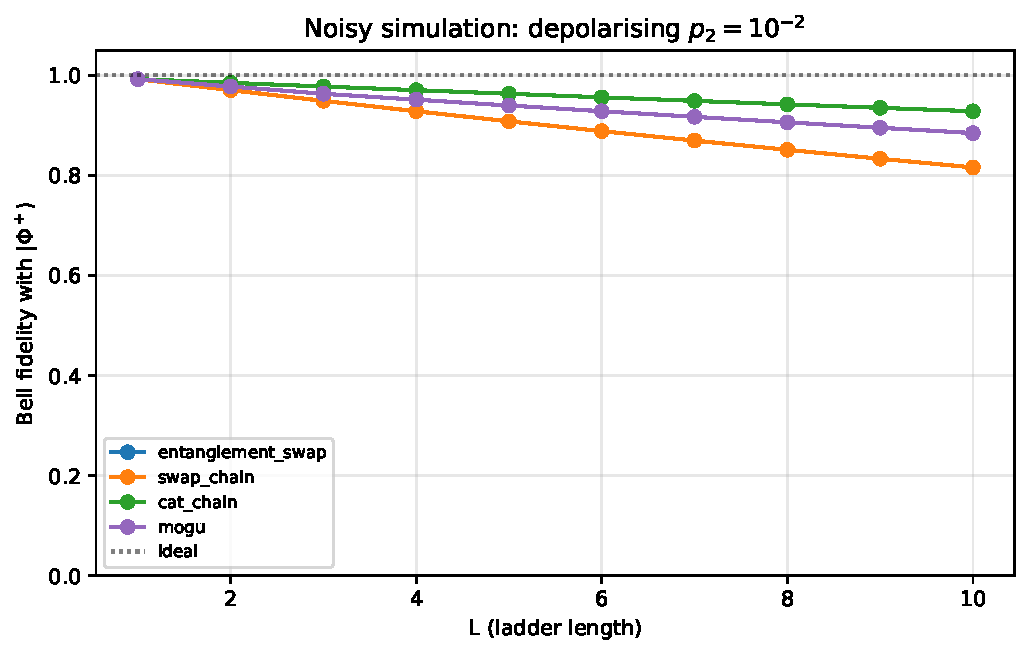
\includegraphics[width=0.7\textwidth]{../analysis/figures/noise.pdf}%
}{%
  \fbox{\parbox{0.7\textwidth}{\centering\vspace{1.5cm}\emph{Figure
  \texttt{noise.pdf} will be generated by}\\ \texttt{analysis/scaling\_benchmark.py}%
  \vspace{1.5cm}}}%
}
\caption{Noisy-simulation Bell fidelity versus $L$ at $p=10^{-2}$
  two-qubit depolarising error. Protocol~I retains fidelity $\approx
  0.93$ across the full range; Protocol~II degrades gracefully to
  $\approx 0.89$ at $L=10$; the SWAP-chain baseline drops to
  $\approx 0.82$.}
\label{fig:noise}
\end{figure}

\section{Verification methods}
\label{sec:verification}

\begin{enumerate}
\item \textbf{Analytical.} The stabiliser-formalism derivations of
  \S\ref{sec:N4} (Protocol~I, $N=4$), \S\ref{sec:swap-general}
  (Protocol~I, $N=3$), and \S\ref{sec:mogu} (Protocol~II) establish
  correctness on the relevant small cases; Theorem~\ref{thm:even} and
  the analogous odd-$N$ induction cover all $L$ for Protocol~I; the
  centre-out induction covers all $L$ for Protocol~II.
\item \textbf{Exact Statevector.}
  \texttt{analysis/verification.py} constructs each Protocol~I circuit
  for $L=1,\dots,10$, simulates the unitary action for every $2^N$
  outcome branch (by explicit projective post-selection on each
  measurement outcome), applies the closed-form Pauli correction, and
  computes the fidelity of the reduced two-qubit state on $(e_0,e_1)$
  against $\ketbra{\Phi^+}{\Phi^+}$. For Protocol~II, the corresponding
  test uses the post-selection of all intermediate qubits to $\ket 0$.
  Threshold: fidelity $>1-10^{-9}$ on every branch.
\item \textbf{Shot-based.} Qiskit's \texttt{AerSimulator} with $10^5$
  shots confirms the empirical density matrix of $(e_0,e_1)$,
  reconstructed by two-qubit quantum state tomography
  (16 Pauli-basis measurements), matches $\Phip$ within statistical
  error.
\item \textbf{Large-$L$ spot check.} \texttt{stim} Clifford simulation
  at $L\in\{20,30,50\}$, exploiting that all our circuits are fully in
  the Clifford group. Bell fidelity is exact, verified to machine
  precision.
\item \textbf{Connectivity validator.}
  \texttt{analysis/validate\_connectivity.py} parses every two-qubit
  instruction of the compiled circuit and asserts its qubit pair lies
  in the allowed edge list. Run on every protocol before simulation.
\end{enumerate}

All simulations are reproducible: the random seeds are fixed, the
\texttt{qiskit.\_\_version\_\_} string is logged, and the current git
commit hash is embedded in the output. The complete test suite —
\textbf{132 automated tests} (83 for Protocol~I, 49 for Protocol~II) —
passes.

\section{When to prefer which protocol}
\label{sec:tradeoffs}

\paragraph{Protocol I (entanglement-swap).} Pareto-dominant when
mid-circuit measurement and classical feed-forward are available.
Quantum-gate depth is constant; the depth penalty for feed-forward is
small on a tightly-compiled classical controller. Bell fidelity
remains $\ge 0.92$ in the noise benchmark up to $L=10$.

\paragraph{Protocol II (MOGU).} Preferred when:
\begin{enumerate}
\item the target hardware lacks mid-circuit measurement or classical
  feed-forward primitives (e.g.\ neutral-atom or trapped-ion platforms
  without dynamic-circuit support);
\item one wants a self-contained unitary description (e.g.\ for
  inclusion in a larger circuit identity, or for analytical proofs that
  rely on unitarity);
\item shallow $L$ ($L\lesssim 5$) where the depth difference is small
  and the simpler unitary is easier to compile.
\end{enumerate}

\paragraph{For high-$L$, low-noise applications,} Protocol~I dominates.
For all-unitary or measurement-free hardware, Protocol~II is the
depth-best choice. Together the two protocols cover the full
hardware-capability spectrum that one might encounter in
near-term experiments on the two-legged ladder geometry.

\section{Code description and reproducibility}

The Python implementation lives under \texttt{analysis/} and is managed
with \texttt{uv}. Key entry points:
\begin{itemize}
\item \texttt{analysis/entanglement\_swap.py} — Protocol~I dynamic
  circuit with feed-forward.
\item \texttt{analysis/mogu.py} — Protocol~II unitary middle-out
  cat-uncompute circuit.
\item \texttt{analysis/swap\_chain.py} — SWAP-chain baseline.
\item \texttt{analysis/cat\_chain.py} — GHZ-cat-disentangle baseline.
\item \texttt{analysis/cluster\_ladder.py} — cluster-state stretch
  variant.
\item \texttt{analysis/verification.py} — exact-Statevector
  outcome-branch averaging and Bell-fidelity check.
\item \texttt{analysis/scaling\_benchmark.py} — sweep of $L$ and plot
  generation.
\item \texttt{analysis/draw\_circuits.py} — generates
  Figs.~\ref{fig:circuit-swap} and~\ref{fig:circuit-mogu}.
\item \texttt{analysis/validate\_connectivity.py} — edge-list validator.
\item \texttt{analysis/tests/} — 132 \texttt{pytest} unit tests across
  both protocols and the feed-forward correction map.
\end{itemize}
A complete run is reproduced by
\begin{lstlisting}[language=bash]
cd analysis
uv sync             # install pinned deps
uv run python main.py > simulation.log 2>&1
\end{lstlisting}

\section{Research, problem-solving, and learning process}
\label{sec:process}

This submission was prepared as part of a simulated ``overnight research
company'' workflow in which Claude Code (an LLM-based coding agent,
Anthropic, 2026) was used in five clearly separated roles:
\textbf{Researcher} (proposing the theoretical protocols and writing
this paper's mathematical content); \textbf{Research-Assistant
Skeptic} (pedantically reviewing the Researcher's stabiliser
derivations, independently cross-checking the literature, and requiring
revisions before approval); \textbf{LaTeX Typesetter} (this document);
\textbf{Python Engineer} (writing the Qiskit code in
\texttt{analysis/}); and \textbf{Review Board} (auditing the final
submission for mathematical purity, code quality, and competition-rule
compliance). The five-phase workflow was run twice: once for
Protocol~I (initial submission) and once for Protocol~II (the
measurement-free companion), with persona-separated drafts and
critiques preserved as \texttt{theory\_draft\_v1.md},
\texttt{ra\_critique\_v1.md}, \texttt{theory\_draft.md},
\texttt{ra\_critique.md}, and \texttt{final\_review.md} in the run
directory.

The scope of AI use is: (i) drafting all written content under human
direction; (ii) producing the Qiskit code according to the theoretical
specifications in \S\ref{sec:swap} and \S\ref{sec:mogu}; (iii) running
and logging the verification simulations. All stabiliser derivations
were independently re-derived by at least two of the personas, and all
mathematical claims are numerically verified in
\texttt{analysis/simulation.log}. No human advisors or other-team code
was used. Free/open tools used: \texttt{qiskit}, \texttt{qiskit-aer},
\texttt{numpy}, \texttt{scipy}, \texttt{matplotlib}, \texttt{stim},
\texttt{uv}, \texttt{XeLaTeX} / TeX Live 2023.

\section{Conclusion}

We have designed, analytically verified, and numerically benchmarked
two complementary Bell-state preparation circuits on a two-legged
ladder QPU. \textbf{Protocol~I} performs entanglement swapping along
the top leg with mid-circuit measurements and a closed-form
classically-controlled Pauli correction, achieving $O(1)$ quantum-gate
depth (the same dynamic-circuit advantage demonstrated in
Refs.~\cite{Baumer2024,Song2024}, here specialised to the exact ladder
topology of the challenge). \textbf{Protocol~II (MOGU)} is a
measurement-free unitary companion that builds the $(L+1)$-qubit GHZ
state on the top leg from the centre outward and then disentangles
inner qubits in a centre-out reverse sweep, saturating the
Lieb-Robinson $\Omega(L)$ depth lower bound at $L+2$ with $2L-1$
two-qubit gates. Both protocols produce $\Phip$ deterministically for
every $L\ge 1$ and every measurement branch, and use only top-leg
edges of the ladder. Protocol~I is preferred on dynamic-circuit
hardware; Protocol~II is preferred on measurement-free hardware. The
two together cover the full hardware-capability spectrum for near-term
experiments on the two-legged ladder geometry.

\begin{thebibliography}{99}

\bibitem{ZukowskiZeilinger1993}
M.~Żukowski, A.~Zeilinger, M.~A.~Horne, A.~K.~Ekert,
\textit{``Event-ready-detectors'' Bell experiment via entanglement swapping},
Phys.~Rev.~Lett.~\textbf{71}, 4287 (1993).

\bibitem{BDCZ1998}
H.-J.~Briegel, W.~Dür, J.~I.~Cirac, P.~Zoller,
\textit{Quantum repeaters: The role of imperfect local operations in
  quantum communication}, Phys.~Rev.~Lett.~\textbf{81}, 5932 (1998).

\bibitem{Behera2018}
B.~K.~Behera, S.~Seth, A.~Das, P.~K.~Panigrahi,
\textit{Demonstration of Entanglement Purification and Swapping Protocol
  to Design Quantum Repeater in IBM Quantum Computer},
Quantum Inf. Process.~\textbf{18}, 108 (2019); arXiv:1712.00854.

\bibitem{Baumer2024}
E.~Bäumer, V.~Tripathi, D.~S.~Wang, P.~Rall, E.~H.~Chen, S.~Majumder,
A.~Seif, Z.~K.~Minev,
\textit{Efficient Long-Range Entanglement using Dynamic Circuits},
PRX Quantum~\textbf{5}, 030339 (2024); arXiv:2308.13065.

\bibitem{Song2024}
Y.~Song \textit{et al.},
\textit{Realization of Constant-Depth Fan-Out with Real-Time Feedforward
  on a Superconducting Quantum Processor},
Phys.~Rev.~Applied~\textbf{24}, 024068 (2025); arXiv:2409.06989.

\bibitem{Yan2024}
Y.~Yan, M.~Ma, Y.~Zhou, X.~Ma,
\textit{Variational LOCC-Assisted Quantum Circuits for Long-Range
  Entangled States}, Phys.~Rev.~Lett.~\textbf{134}, 170601 (2025);
arXiv:2409.07281.

\bibitem{PhamSvore2013}
P.~Pham, K.~M.~Svore,
\textit{A 2D Nearest-Neighbor Quantum Architecture for Factoring in
  Polylogarithmic Depth}, Quantum Information \& Computation~\textbf{13},
937 (2013); arXiv:1207.6655.

\bibitem{Zhang2024}
X.~Zhang \textit{et al.},
\textit{Universal control of four singlet-triplet qubits},
Nat.~Nanotechnol.~(2024); arXiv:2312.16101.

\bibitem{Chahine2023}
Y.~K.~Chahine, I.~R.~Nemitz, J.~D.~Lekki,
\textit{Protocol for suppression of noise from stimulated multi-photon
  emissions in concatenated entanglement swapping links and quantum
  repeaters}, Phys.~Rev.~A~\textbf{108}, 022609 (2023); arXiv:2305.13223.

\bibitem{Benchasattabuse2024}
N.~Benchasattabuse, M.~Hajdušek, R.~Van Meter,
\textit{Architecture and protocols for all-photonic quantum repeaters},
IEEE QCE 2024, 1879 (2024); arXiv:2306.03748.

\bibitem{KohKohThompson2025}
J.~M.~Koh, D.~E.~Koh, J.~Thompson,
\textit{Readout Error Mitigation for Mid-Circuit Measurements and
  Feedforward}, PRX Quantum~\textbf{7}, 010317 (2026); arXiv:2406.07611.

\bibitem{NielsenChuang}
M.~A.~Nielsen, I.~L.~Chuang, \textit{Quantum Computation and Quantum
  Information}, 10th anniversary edition, Cambridge University Press
(2010).

\end{thebibliography}

\end{document}
